\documentclass[12pt]{article}
\usepackage{graphicx}
\usepackage{float}
\begin{document}
\title{Statistics 12, Lab 3}
\date{February 19th, 2019}
\author{Michael Wu\\UID: 404751542}
\maketitle

\section*{Exercise 1}

\paragraph{a)}

I ran the following code.
\begin{verbatim}
linear_model <- lm(soil$lead ~ soil$zinc)
summary(linear_model)
\end{verbatim}
This output the following statistics.
\begin{verbatim}
Call:
lm(formula = soil$lead ~ soil$zinc)

Residuals:
    Min      1Q  Median      3Q     Max
-79.853 -12.945  -1.646  15.339 104.200

Coefficients:
             Estimate Std. Error t value Pr(>|t|)
(Intercept) 17.367688   4.344268   3.998 9.92e-05 ***
soil$zinc    0.289523   0.007296  39.681  < 2e-16 ***
---
Signif. codes:  0 ‘***’ 0.001 ‘**’ 0.01 ‘*’ 0.05 ‘.’ 0.1 ‘ ’ 1

Residual standard error: 33.24 on 153 degrees of freedom
Multiple R-squared:  0.9114,	Adjusted R-squared:  0.9109
F-statistic:  1575 on 1 and 153 DF,  p-value: < 2.2e-16
\end{verbatim}

\paragraph{b)}

I ran the following code.
\scriptsize
\begin{verbatim}
plot(soil$lead ~ soil$zinc, xlab="Zinc Concentration (ppm)",
     ylab="Lead Concentration (ppm)", main="Lead vs. Zinc in Soil")
abline(linear_model, col="red", lwd=2)
\end{verbatim}
\normalsize
This generated the following plot.
\begin{figure}[H]
    \begin{center}
        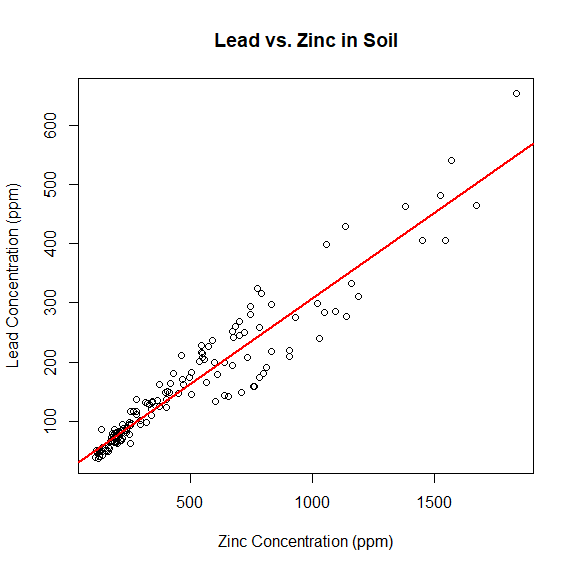
\includegraphics[width=4.5in]{exercise1b.png}
    \end{center}
\end{figure}

\paragraph{c)}

I ran the following code
\scriptsize
\begin{verbatim}
plot(linear_model$residuals ~ soil$zinc, xlab="Zinc Concentration (ppm)",
     ylab="Lead Residuals (ppm)", main = "Lead vs. Zinc in Soil Residuals plot")
abline(a=0, b=0, col="red", lwd=2)
\end{verbatim}
\normalsize
This generated the following plot.
\begin{figure}[H]
    \begin{center}
        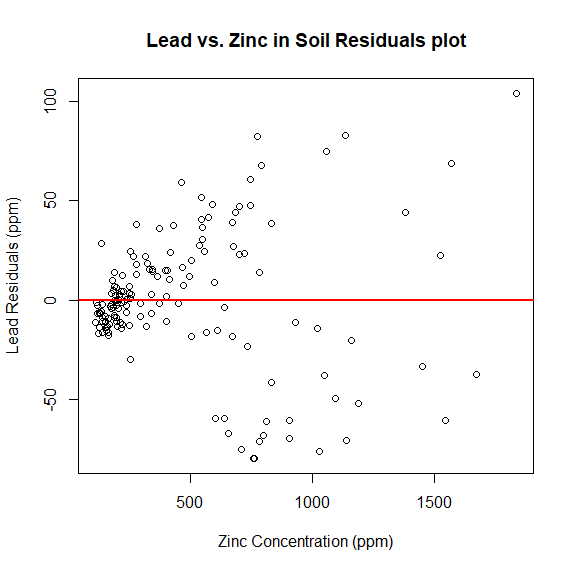
\includegraphics[width=4.5in]{exercise1c.png}
    \end{center}
\end{figure}

\paragraph{d)}

The equation of the regression line is the following.
\[y=0.289523x+17.367688\]

\paragraph{e)}

We would expect the lead concentration to be 306.89 ppm.

\paragraph{f)}

We would expect the lead concentration to be 28.95 ppm higher.

\paragraph{g)}

The R-squared value is 0.9114. In this context it means that 91.14\% of
the variation in the lead concentration can be determined by the variation in zinc
concentration.

\paragraph{h)}

I believe that linearity, symmetry, and are met for this data. The data appears
very straight and the residuals look symmetrical. However,
the condition for equal variance is not met. The residuals appear to become
more spread out as the zinc concentration becomes greater. This would indicate
that our model does not capture all the details of our system. Perhaps of the
logarithms of both zinc and lead would be more appropriate to compare with each other.

\section*{Exercise 2}

\paragraph{a)}

I ran the following code.
\begin{verbatim}
linear_model2 <- lm(ice$Extent ~ ice$Date)
summary(linear_model2)
\end{verbatim}
This output the following statistics.
\begin{verbatim}
Call:
lm(formula = ice$Extent ~ ice$Date)

Residuals:
   Min     1Q Median     3Q    Max
-9.445 -5.439  1.442  5.599  7.564

Coefficients:
             Estimate Std. Error t value Pr(>|t|)
(Intercept) 1.011e+01  1.558e+00   6.486 4.11e-10 ***
ice$Date    1.438e-04  1.411e-04   1.019    0.309
---
Signif. codes:  0 ‘***’ 0.001 ‘**’ 0.01 ‘*’ 0.05 ‘.’ 0.1 ‘ ’ 1

Residual standard error: 5.654 on 273 degrees of freedom
Multiple R-squared:  0.003787,	Adjusted R-squared:  0.0001377
F-statistic: 1.038 on 1 and 273 DF,  p-value: 0.3093
\end{verbatim}

\paragraph{b)}

I ran the following code.
\scriptsize
\begin{verbatim}
plot(ice$Extent ~ ice$Date, xlab="Date (Year)",
     ylab="Ice Extent (millions of km^2)", main="Ice Extent Over Time", type="l")
abline(linear_model2, col="red", lwd=2)
\end{verbatim}
\normalsize
This generated the following plot.
\begin{figure}[H]
    \begin{center}
        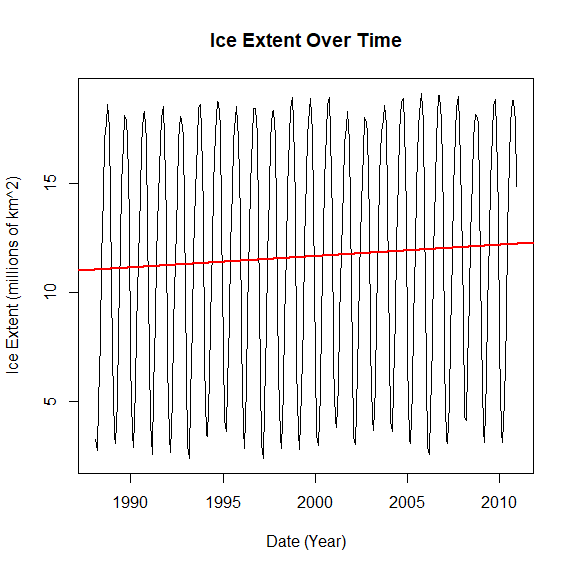
\includegraphics[width=4.5in]{exercise2b.png}
    \end{center}
\end{figure}
There does seem to be a slight upwards trend in this data as shown by the regression line.
However, the main change in sea ice extent seems to come from the change in the seasons. The
sea periodically rises and falls with a period of a year.

\paragraph{c)}

I ran the following code
\scriptsize
\begin{verbatim}
plot(linear_model2$residuals ~ ice$Date, xlab="Date (Year)",
     ylab="Ice Extent Residuals (millions of km^2)",
     main = "Ice Extent Over Time Residuals plot")
abline(a=0, b=0, col="red", lwd=2)
\end{verbatim}
\normalsize
This generated the following plot.
\begin{figure}[H]
    \begin{center}
        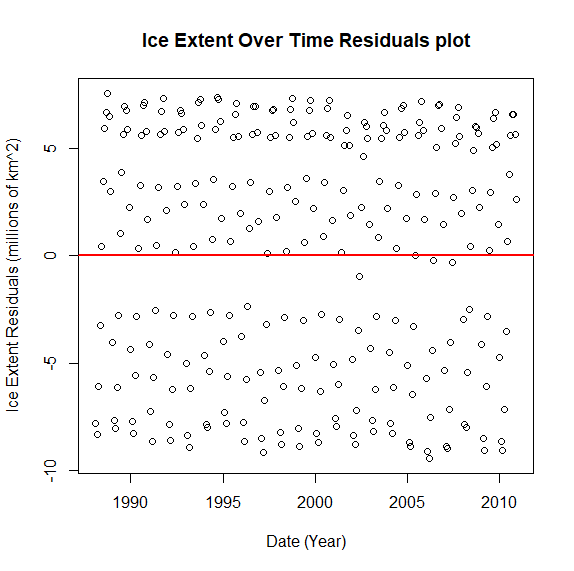
\includegraphics[width=4.5in]{exercise2c.png}
    \end{center}
\end{figure}
The assumption about the model that we should be concerned about is the linearity
assumption. The residuals have bands where the density changes, which indicates
that our model consistently over and under predicts the sea ice extent within certain
time frames. In reality the sea ice extent is probably best modeled by a
sinusoidal relationship. If we want a linear model we could also take the average
ice size over the year or only record the ice size during a specific season.

\section*{Exercise 3}

\paragraph{a)}

There is an \(\frac{8}{36}\) chance that Adam will double his money in the first
round of the game and a \(\frac{4}{36}\) chance that Adam will lose his money
in the first round of the game.

\paragraph{b)}

I ran the following code.
\begin{verbatim}
set.seed(123)
faces = 1:6
rolls = do(5000) * sample(faces, 2, replace=TRUE)
sums = rowSums(rolls)
\end{verbatim}
The first five sums that were generated were 9, 7, 10, 7, and 9.

\paragraph{c)}

I ran the following code.
\scriptsize
\begin{verbatim}
histogram(sums, main="Sum of Two Fair Six-Sided Dice Rolls",
        xlab="Sum", ylab="Times Rolled", n=11, type="count")
\end{verbatim}
\normalsize
This generated the following plot.
\begin{figure}[H]
    \begin{center}
        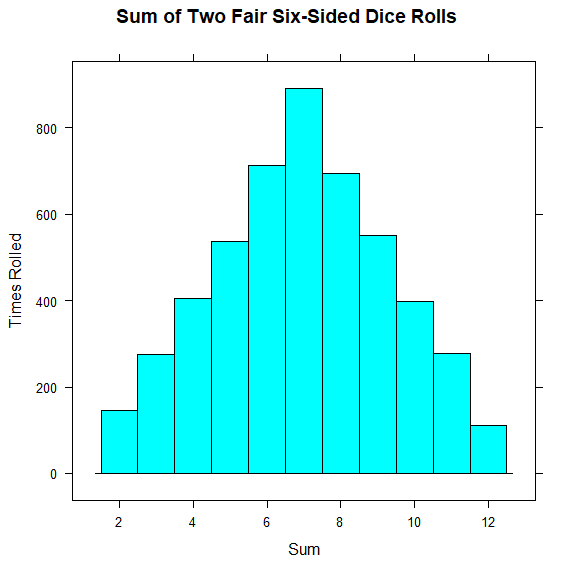
\includegraphics[width=4.5in]{exercise3c.png}
    \end{center}
\end{figure}

\paragraph{d)}

I ran the following code.
\begin{verbatim}
mean(sums == 7 | sums == 11)
mean(sums == 2 | sums == 3 | sums == 12)
\end{verbatim}
This output that Adam doubled his money 23.36\% of the time in the simulation and lost
his money 10.64\% of the time in the simulation.

\paragraph{e)}

They are mutually exclusive and not independent. This is because Adam cannot
both win money and lose money on the first round at the same time. If they
were independent, the probability of both events happening would be nonzero and
equal to the product of the probabilities of the two independent events.

\paragraph{f)}

Let's assume that event \(A\) is Adam doubling his money and event \(B\) is
Adam losing his money. Assume for contradiction that \(A\) and \(B\) are independent.
Then we have the following.
\[P(A\cap B)=P(A)P(B)=\frac{8}{36}\frac{4}{36}=\frac{2}{81}\]
But we know that \(P(A\cap B)=0\), a contradiction. Thus \(A\) and \(B\) are not
independent.

\section*{Exercise 4}

\paragraph{a)}

\paragraph{b)}

\paragraph{c)}

\paragraph{d)}

\paragraph{e)}

\end{document}